\chapter{Simplex theory}

In this section, we present the various definitions connected
to simplex algorithms. We introduce several methods to measure 
the size of a simplex, including the oriented length. 
We present several methods to compute an
initial simplex, that is, the regular simplex used by Spendley et al.,
the axis-by-axis simplex, Pfeffer's simplex and the randomized 
bounds simplex.
%We also present the simplex gradient, which is a forward or a centered 
%difference formula for the gradient of the cost function.
%The core of this section is from \cite{Kelley1999}.

\section{The simplex}

\begin{definition}
(\emph{Simplex})
A \emph{simplex} $S$ in $\RR^n$ is the convex hull of $n+1$ vertices, that is, 
a simplex $S=\{\bv_i\}_{i=1,n+1}$ is defined 
by its $n+1$ vertices $\bv_i \in \RR^n$ for $i=1,n+1$.
\end{definition}

The $j$-th coordinate of the $i$-th vertex $\bv_i\in\RR^n$ is denoted  
by $(\bv_i)_j\in\RR$.

Box extended the Nelder-Mead algorithm to handle bound and non linear constraints \cite{Box1965}.
To be able to manage difficult cases, he uses a \emph{complex} made of $m\geq n+1$ vertices.

\begin{definition}
(\emph{Complex})
A \emph{complex} $S$ in $\RR^n$ is a set of $m\geq n+1$ vertices, that is, 
a simplex $S=\{\bv_i\}_{i=1,m}$ is defined 
by its $m$ vertices $\bv_i \in \RR^n$ for $i=1,m$.
\end{definition}

In this chapter, we will state clearly when the definition and results can only be applied 
to a simplex or to a more general a complex. 
%Indeed, some definitions such as the simplex gradient cannot be extended to a \emph{complex}
%and are only applicable to a \emph{simplex}.

We assume that we are given a cost function $f:\RR^n\rightarrow\RR$.
Each vertex $\bv_i$ is associated with a function value $f_i = f(\bv_i)$ for $i=1,m$.
For any complex, the vertices can be sorted by increasing function values 
\begin{eqnarray}
\label{simplex-sortedfv}
f_1 \leq f_2 \leq \ldots \leq f_n \leq f_m.
\end{eqnarray}

The sorting order is not precisely defined neither in Spendley's et al paper \cite{Spendley1962}
nor in Nelder and Mead's \cite{citeulike:3009487}. 
In \cite{lagarias:112}, the sorting rules are defined precisely to be able to 
state a theoretical convergence result. In practical implementations, though, the 
ordering rules have no measurable influence.

For a given simplex $S$, let $V$ denote the 
$n\times n$ matrix of simplex directions 
\begin{eqnarray}
\label{simplex-directions}
V(S) = (\bv_2 - \bv_1, \bv_3 - \bv_1 , \ldots , \bv_{n+1} - \bv_1).
\end{eqnarray}

We say that the simplex $S$ is nonsingular if the matrix of simplex directions $V(S)$ is nonsingular.

\section{The size of the complex}
\label{section-simplexsize}

Several methods are available to compute the size of a complex.

In this section, we use  the euclidian norm $\|.\|_2$ 
the defined by 
\begin{eqnarray}
\|\bv\|_2 = \sum_{j=1,n}(v_j)^2.
\end{eqnarray}

\begin{definition}
(\emph{Diameter})
The simplex diameter $diam(S)$ is defined by 
\begin{eqnarray}
\label{simplex-diameter}
diam(S) = \max_{i,j=1,m} \|\bv_i - \bv_j\|_2.
\end{eqnarray}
\end{definition}

In practical implementations, computing the diameter 
requires two nested loops over the 
vertices of the simplex, i.e. requires $m^2$ 
operations. This is why authors generally 
prefer to use lengths which are less expensive 
to compute.

\begin{definition}
(\emph{Oriented length})
The two oriented lengths $\sigma_-(S)$ and 
$\sigma_+(S)$ are defined by 
\begin{eqnarray}
\label{simplex-sigma}
\sigma_+(S) = \max_{i=2,m} \|\bv_i - \bv_1\|_2 
\qquad \textrm { and } \qquad \sigma_-(S) = \min_{i=2,m} \|\bv_i - \bv_1\|_2.
\end{eqnarray}
\end{definition}

\begin{proposition}
The diameter and the maximum oriented length
satisfy the following inequalities 
\begin{eqnarray}
\label{simplex-sigma-diam}
\sigma_+(S) \leq diam(S) \leq 2 \sigma_+(S).
\end{eqnarray}
\end{proposition}

\begin{proof}
We begin by proving that
\begin{eqnarray}
\sigma_+(S) \leq diam(S).
\end{eqnarray}
This is directly implied by the inequality
\begin{eqnarray}
\max_{i=2,m} \|\bv_i - \bv_1\|_2
&\leq& \max_{i=1,m} \|\bv_i - \bv_1\|_2 \\
&\leq& \max_{i,j=1,m} \|\bv_i - \bv_j\|_2,
\end{eqnarray}
which concludes the first part of the proof.
We shal now proove the inequality 
\begin{eqnarray}
\label{eq-simplex-ineqdiam}
\diam(S) \leq 2 \sigma_+(S).
\end{eqnarray}
We decompose the difference 
$\bv_i - \bv_j$ into 
\begin{eqnarray}
\bv_i - \bv_j = (\bv_i - \bv_1)+(\bv_1 - \bv_j).
\end{eqnarray}
Hence,
\begin{eqnarray}
\| \bv_i - \bv_j\|_2 \leq \|\bv_i - \bv_1\|_2
+\| \bv_1 - \bv_j\|_2.
\end{eqnarray}
We take the maximum over $i$ and $j$,
which leads to
\begin{eqnarray}
\max_{i,j=1,m}\| \bv_i - \bv_j\|_2 
&\leq& \max_{i=1,m}\|\bv_i - \bv_1\|_2 
+\max_{j=1,m}\| \bv_1 - \bv_j\|_2 \\
&\leq& 2 \max_{i=1,m}\|\bv_i - \bv_1\|_2.
\end{eqnarray}
With the definitions of the diameter
and the oriented length, this immediately 
prooves the inequality 
\ref{eq-simplex-ineqdiam}.
end{proof}

In Nash's book \cite{nla.cat-vn1060620}, the size of the simplex $s_N(S)$ is measured
based on the 1-norm and is defined by 
\begin{eqnarray}
\label{simplex-sizenash}
s_N(S) = \sum_{i=2,m} \|\bv_i - \bv_1\|_1
\end{eqnarray}
where the 1-norm is defined by 
\begin{eqnarray}
\label{simplex-sizenash2}
\|\bv_i \|_1 = \sum_{j=1,n} |(\bv_i)_j|.
\end{eqnarray}

\section{The initial simplex}

While most of the theory can be developed without being very specific 
about the initial simplex, it plays a very important role in practice.
All approaches are based on the initial guess $\bx_0\in\RR^n$ and create a 
geometric shape based on this point.

In this section, we present the various approach to design the initial 
simplex. In the first part, we emphasize the importance of the initial
simplex in optimization algorithms. Then we present the regular simplex 
by Spendley et al., the axis-by-axis simplex, the randomized bounds approach by Box and 
Pfeffer's simplex.

\subsection{Importance of the initial simplex}

The initial simplex is particularily important in the case of Spendley's et al 
method, where the shape of the simplex is fixed during the iterations.
Therefore, the algorithm can only go through points which are on the pattern
defined by the initial simplex. The pattern presented in figure \ref{fig-nm-simplex-fixedshape}
is typical a fixed-shape simplex algorithm (see \cite{Torczon89multi-directionalsearch}, chapter 3, 
for other patterns of a direct search method).
If, by chance, the pattern is so that the optimum is close to one point 
defined by the pattern, the number of iteration may be small. On the contrary, the 
number of iterations may be large if the pattern does not come close to the 
optimum.

\begin{figure}
\begin{center}
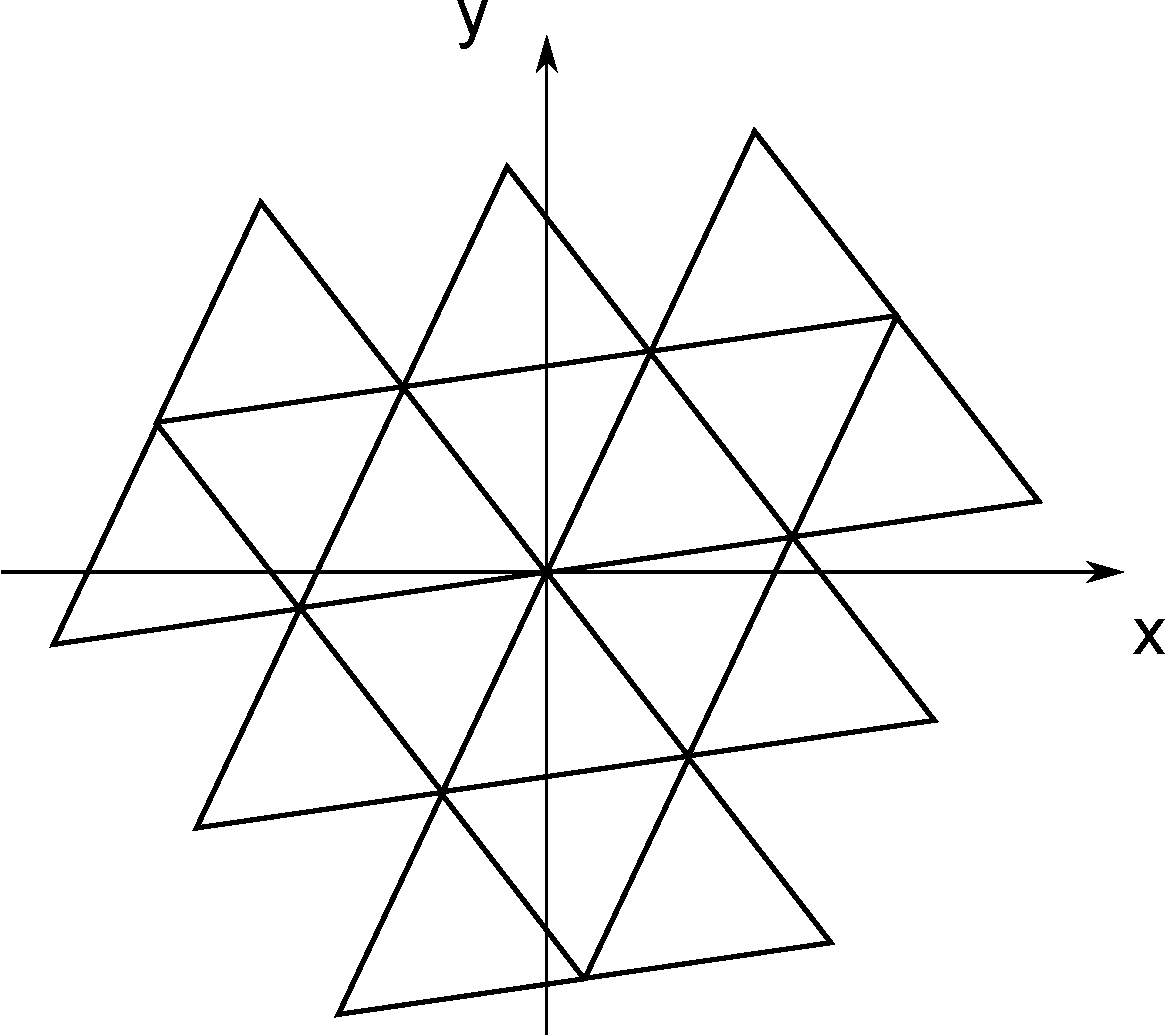
\includegraphics[width=7cm]{simplex_initialfixed.pdf}
\end{center}
\caption{Typical pattern with fixed-shape Spendley's et al algorithm}
\label{fig-nm-simplex-fixedshape}
\end{figure}

The variable-shape simplex algorithm designed by Nelder and Mead is also very
sensitive to the initial simplex.
One of the problems is that the initial simplex should be consistently scaled 
with respect to the unknown $\bx$.
In "An investigation into the efficiency of variants on the simplex method" \cite{parkinson1972}, 
Parkinson and Hutchinson explored 
several improvements of Nelder and Mead's algorithm. First, they investigate the sensitivity
of the algorithm to the initial simplex. Two parameters were investigated,
that is, the initial length and the orientation of the simplex. 
The conclusion of their study with respect to the initial simplex is 
the following. "The orientation of the initial simplex has a significant effect 
on efficiency, but the relationship can be too sensitive for an automatic 
predictor to provide sufficient accuracy at this time."

Since no initial simplex clearly improves on the others, in practice, 
it may be convenient to try different approaches.

\subsection{Spendley's et al regular simplex}

In their paper \cite{Spendley1962}, Spendley et al. use a regular 
simplex with given size $\ell>0$. We define the parameters $p,q>0$ as 
\begin{eqnarray}
p &=& \frac{1}{n\sqrt{2}} \left(n-1 + \sqrt{n+1}\right), \\
q &=& \frac{1}{n\sqrt{2}} \left(\sqrt{n+1} - 1\right).
\end{eqnarray}
We can now define the vertices of the simplex $S=\{\bx_i\}_{i=1,n+1}$.
The first vertex of the simplex is the initial guess 
\begin{eqnarray}
\bv_1 &=& \bx_0.
\end{eqnarray}
The other vertices are defined by 
\begin{eqnarray}
(\bv_i)_j &=& 
\left\{
\begin{array}{l}
(\bx_0)_j + \ell p, \textrm{ if } j=i-1,\\
(\bx_0)_j + \ell q, \textrm{ if } j\neq i-1,\\
\end{array}
\right.
\end{eqnarray}
for vertices $i=2,n+1$ and components $j=1,n$, 
where $\ell \in\RR$ is the length of the simplex and satisfies $\ell>0$. Notice that this 
length is the same for all the edges which keeps the simplex regular.

The regular simplex is presented in figure \ref{fig-nm-simplex-regular}.

\begin{figure}
\begin{center}
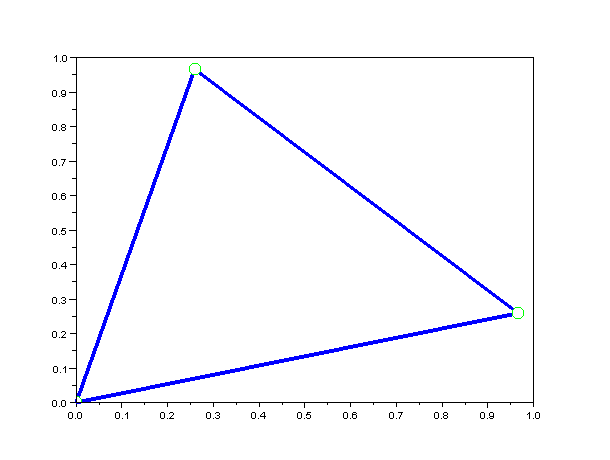
\includegraphics[width=10cm]{simplex_regular.png}
\end{center}
\caption{Regular simplex in 2 dimensions}
\label{fig-nm-simplex-regular}
\end{figure}

\subsection{Axis-by-axis simplex}

A very efficient and simple approach leads to an axis-by-axis simplex.
This simplex depends on a vector of positive lengths $\bl\in\RR^n$.
The first vertex of the simplex is the initial guess 
\begin{eqnarray}
\bv_1 &=& \bx_0.
\end{eqnarray}
The other vertices are defined by 
\begin{eqnarray}
(\bv_i)_j &=& 
\left\{
\begin{array}{l}
(\bx_0)_j + \ell_j, \textrm{ if } j=i-1,\\
(\bx_0)_j, \textrm{ if } j\neq i-1,\\
\end{array}
\right.
\end{eqnarray}
for vertices $i=2,n+1$ and components $j=1,n$.

This type of simplex is presented in figure \ref{fig-nm-simplex-axes},
where $\ell_1=1$ and $\ell_2=2$.
The axis-by-axis simplex is used in the Nelder-Mead 
algorithm provided in Numerical Recipes in C \cite{NumericalRecipes}.
As stated in \cite{NumericalRecipes}, the length vector $\bl$ can 
be used as a guess for the characteristic length scale of the problem.

\begin{figure}
\begin{center}
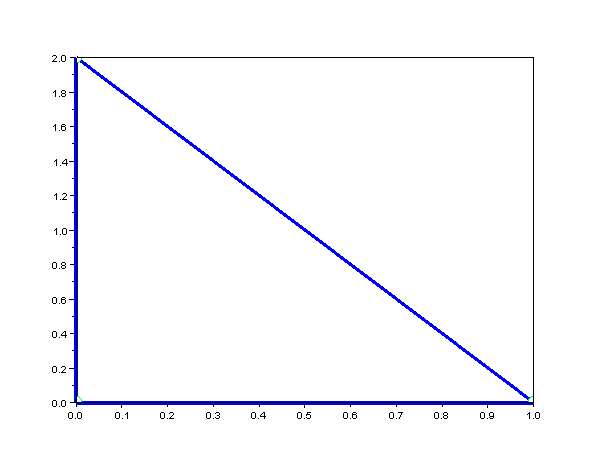
\includegraphics[width=10cm]{simplex_axes.png}
\end{center}
\caption{Axis-based simplex in 2 dimensions -- Notice that the length along the $x$ axis is 1 while the length
along the $y$ axis is 2. }
\label{fig-nm-simplex-axes}
\end{figure}

\subsection{Randomized bounds}

Assume that the variable $\bx\in\RR^n$ is bounded so that 
\begin{eqnarray}
m_j \leq x_j \leq M_j,
\end{eqnarray}
for $j=1,n$, where $m_j,M_j\in\RR$ are minimum 
and maximum bounds and $m_j\leq M_j$.
A method suggested by Box in \cite{Box1965} is 
based on the use of 
pseudo-random numbers. Let 
$\{\theta_{i,j}\}_{i=1,n+1,j=1,n}\in[0,1]$ be 
a sequence of random numbers uniform in the 
interval $[0,1]$.
The first vertex of the simplex is the initial guess 
\begin{eqnarray}
\bv_1 &=& \bx_0.
\end{eqnarray}
The other vertices are defined by 
\begin{eqnarray}
(\bv_i)_j &=& m_j + \theta_{i,j} (M_j - m_j),
\end{eqnarray}
for vertices $i=2,n+1$ and components $j=1,n$.

\subsection{Pfeffer's method}

This initial simplex is used in the function \scifunction{fminsearch}
and presented in \cite{Fan2002}. According to \cite{Fan2002}, this simplex is due to L. Pfeffer at Stanford.
The goal of this method is to scale the initial simplex with respect 
to the characteristic lengths of the problem. This allows, for example,
to manage cases where $x_1\approx 1$ and $x_2\approx 10^5$.
As we are going to see, the scaling is defined with respect to the 
initial guess $\bx_0$, with an axis-by-axis method.

The method proceeds by defining $\delta_u,\delta_z>0$, where 
$\delta_u$ is used for usual components of $\bx_0$ and $\delta_z$ is 
used for the case where one component of $\bx_0$ is zero.
The default values for $\delta_u$ and $\delta_z$ are 
\begin{eqnarray}
\delta_u = 0.05 \qquad \textrm{and} \qquad \delta_z = 0.0075.
\end{eqnarray}
The first vertex of the simplex is the initial guess 
\begin{eqnarray}
\bv_1 &=& \bx_0.
\end{eqnarray}
The other vertices are defined by 
\begin{eqnarray}
(\bv_i)_j &=& \left\{
\begin{array}{l}
(\bx_0)_j + \delta_u (\bx_0)_j, \textrm{ if } j=i-1 \textrm{ and } (\bx_0)_{j-1}\neq 0,\\
\delta_z, \textrm{ if } j=i-1 \textrm{ and } (\bx_0)_{j-1}= 0,\\
(\bx_0)_j, \textrm{ if } j\neq i-1,\\
\end{array}
\right.
\end{eqnarray}
for vertices $i=2,n+1$ and components $j=1,n$.

%\section{The simplex gradient}
%\label{section-simplexgradient}

%TODO...

\section{References and notes}

Some elements of the section \ref{section-simplexsize} is taken from 
Kelley's book \cite{Kelley1999}, "Iterative Methods for Optimization".
While this document focus on Nelder-Mead algorithm, Kelley gives a broad
view on optimization and present other algorithms for noisy functions,
like implicit filtering, multidirectional search and the Hooke-Jeeves algorithm.